
\section{Problem 3}

\begin{quoting}
  For this exercise, you will follow Chapter 11 of the Imbens and
  Rubin textbook, but use a different data set to implement some of
  the techniques we have learned about in class. While the textbook
  describes analysis of a social program called the Saturation Work
  Initiative Model (SWIM) program, in this exercise you will analyze
  the lalonde data available in the \textsf{R} package
  \texttt{MatchIt} with the command \texttt{data(lalonde)}. Use the
  \texttt{help(lalonde)} command to get a basic description of the
  data. Use the variable called \texttt{treat} to denote the
  randomized treatment assignment, and use \texttt{re78} as the
  outcome of interest.
\end{quoting}

\begin{enumerate}[(a)]
  % -------------------------------------------------------------------------
  % A
\item
  \begin{quoting}
    Produce a table analogous to Table 11.2 of the textbook. Use the
    same test statistics as in Section 11.3, and conduct the tests for
    the entire data set (corresponding to the All column in Table 11.2)
    and stratified by the \texttt{nodegree} variable (corresponding to
    the two rightmost columns of Table 11.2).
    % -------------------------------------------------------------------------
  \end{quoting}
  See Table~\ref{tab:fisher-test} for $p$-values corresponding to
  these tests.  The null distributions and observed test statistics
  are shown in Figure~\ref{fig:fisher-hist}.
  \begin{table}
    \centering
    \begin{tabular}[]{ l r r r}\toprule
      Statistics        & All      & No High School Degree & High School Degree \\
                        & (614)    & (387)                 & (227)              \\
      \midrule
      $T^{\rank}$       & $0.282$  & $0.420$               & $0.791$            \\
      $T^{\rank-\gain}$ & $<0.000$ & $0.007$               & $0.005$            \\
      $T^{\dif}$        & $0.336$  & $0.499$               & $0.888$            \\
      \bottomrule
    \end{tabular}
    \caption{\label{tab:fisher-test} Fisher exact tests for the sharp
      null hypothesis $H_0: Y_i(1) - Y_i(0) = 0$ for the Lalonde
      dataset. }
  \end{table}
  \begin{figure}[]
    \centering
    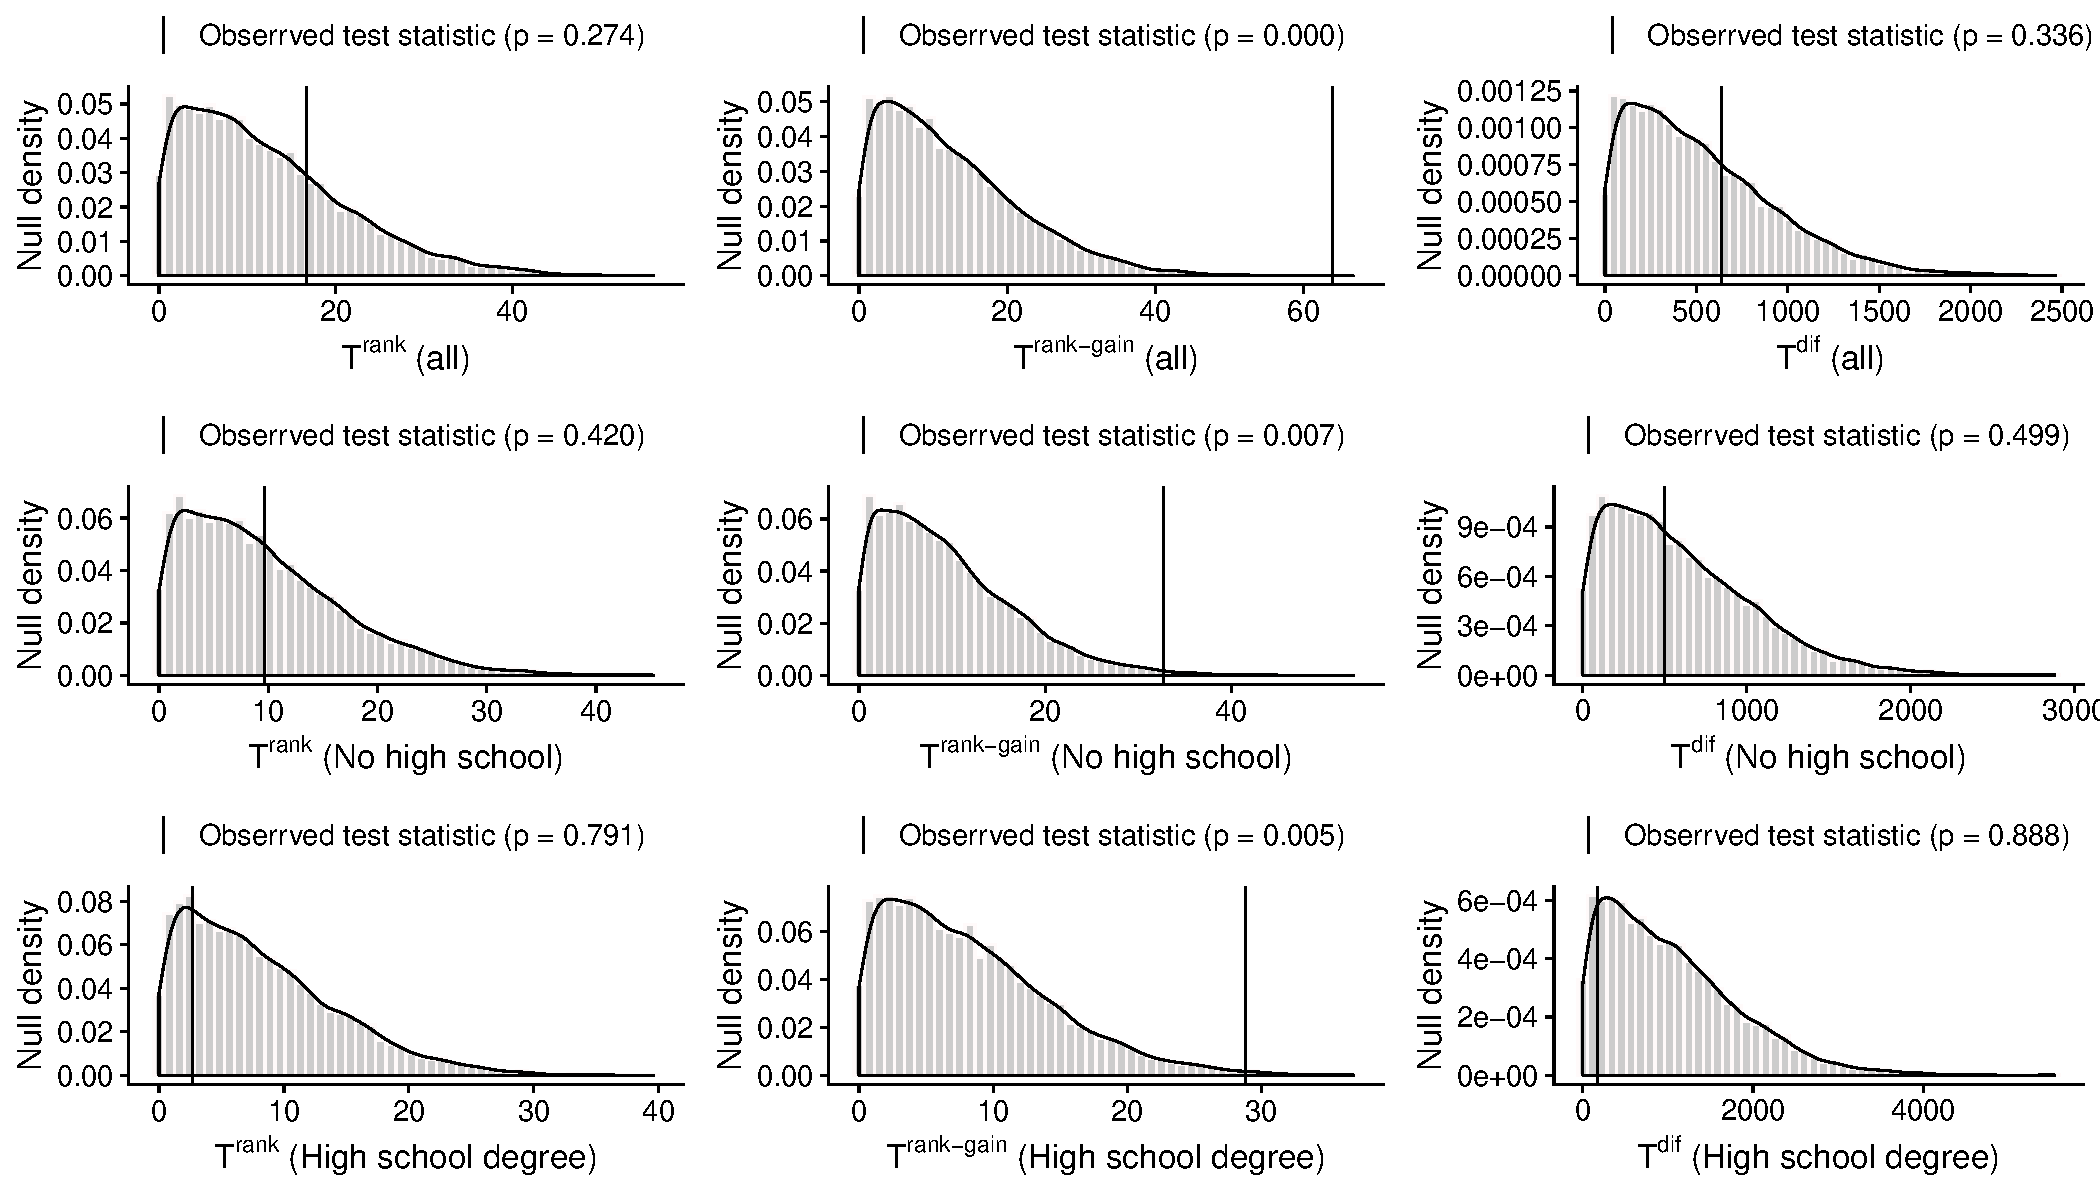
\includegraphics[width=0.9\textheight, angle = 90]{figures/hist-all.pdf}
    \caption{Null distributions, observed test statistics, and
      $p$-values corresponding to comparisons made in
      Table~\ref{tab:fisher-test}.}
    \label{fig:fisher-hist}
  \end{figure}

  % -------------------------------------------------------------------------
  % B
\item
  \begin{quoting}
    Unlike in Section 11.3 of the textbook, provide a Fisher interval
    for the analysis of the entire data set (i.e., not stratified by
    \texttt{nodegree}).
  \end{quoting}
  Note that we can determine confidence intervals from inverting a
  series of hypothesis tests $H_{0}^C: Y_i(1) - Y_i(0) = C$.  That is,
  the confidence interval is the set of values of $C$ for which we
  fail to reject $H^C_0$.  Here are three (approximate) 95\%
  confidence intervals resulting from the tests given in Part (a).
  \begin{align*}
    T^{\text{Rank}}:\;\;\;& (-1050, 0) \\
    T^{\text{Rank-Gain}}:\;\;\;& (1000, 3250) \\
    T^{\text{dif}}:\;\;\;&  (-1877.55, 693.88)
  \end{align*}
  The interval coming from the rank test includes zero because the
  presence of many 0's in $Y^{\obs}$ leads to the test being very
  sensitive to small perturbations of $C$. 
  % -------------------------------------------------------------------------
  % C
\item
  \begin{quoting}
    Produce a table analogous to Table 11.3 of the textbook, but with
    estimates for the same three categories as in part (a) (All and
    both levels of \texttt{nodegree}).
  \end{quoting}
  See Table~\ref{tab:neyman}.
  \begin{table}[ht!]
    \centering
    \begin{tabular}{l|rrr}
      \toprule
                                & All      & No High School Degree & High School Degree \\
                                & (614)    & (387)                 & (227)              \\ \midrule
      Est                       & --635.03 & --497.615             & --176.36           \\
      $(\widehat{\text{s.e.})}$ & 677.20   & 774.94                & 1317.78            \\ 
      \bottomrule
    \end{tabular}
    \caption{\label{tab:neyman}Estimates for average treatment effects on earnings from
      the Lalonde dataset based on Neyman's repeated sampling approach.
    }
  \end{table}
  % -------------------------------------------------------------------------
  % D
\item 
  \begin{quoting}
    Fit a regression model with interactions as in Section 11.5 of the
    textbook, using the following variables as covariates:
    \texttt{age}, \texttt{educ}, \texttt{black}, \texttt{hispan},
    \texttt{married}, \texttt{nodegree}.  Report the population
    average treatment effect from this model and compare it with the
    effect estimates from a regression model that adjusts only for the
    treatment indicator.
  \end{quoting}
  \begin{table}[]
    \centering
    \begin{tabular}{l|rr|rr}
      \toprule
      \textit{Covariates}                                & Est    & $\widehat{\text{s.e.}}$ & Est       & $\widehat{\text{s.e.}}$ \\ \midrule
      \texttt{intercept}                     &   6984.17  & 360.71                          & 6404.82   & 391.99                  \\
      \texttt{treatment}                      &  --635.03 & 657.14                          & 863.07    & 1040.78                 \\ \midrule
      \texttt{age}                                       &        &                         & 48.26     & 36.44                   \\
      \texttt{educ}                                      &        &                         & 526.20    & 188.29                  \\
      \texttt{black}                                     &        &                         & --1672.81 & 923.90                  \\
      \texttt{hispan}                                    &        &                         & 723.87    & 1059.16                 \\
      \texttt{married}                                   &        &                         & 2369.01   & 786.56                  \\
      \texttt{nodegree}                                  &        &                         & 213.62    & 1064.92                 \\
                                                         &        &                         &           &                         \\
      \textit{Interactions with treatment}               &        &                         &           &                         \\ \midrule
      \texttt{treat} $\times$ \texttt{age}               &        &                         & 34.04     & 86.79                   \\
      \texttt{treat} $\times$ \texttt{educ}              &        &                         & 102.78    & 411.75                  \\
      \texttt{treat} $\times$ \texttt{black}             &        &                         & 598.43    & 2049.87                 \\
      \texttt{treat} $\times$ \texttt{hispan}            &        &                         & --263.67  & 3020.45                 \\
      \texttt{treat} $\times$ \texttt{married}           &        &                         & --1028.01 & 1621.14                 \\
      \texttt{treat} $\times$ \texttt{nodegree}          &        &
                                                                                            & --591.56  & 1947.89                 \\ \bottomrule
    \end{tabular}
    \caption{\label{tab:reg-table} Regression analyses for the Lalonde
      dataset, with and without covariates and treatment
      interactions. }
  \end{table}
  See Table~\ref{tab:reg-table}.  Note that the regression without
  covariates returns a negative point estimate for the treatment
  effect, while the regression with covariates returns a positive
  point estimate for the treatment effect.  However, neither estimate
  is statistically significant at the $\alpha = 0.1$ level.  
  % -------------------------------------------------------------------------
  % E
\item
  \begin{quoting}
    The second paragraph of Section 11.6 describes an analysis
    assuming a normal distribution for the two potential outcomes with
    the correlation between $Y_i(0)$ and $Y_i(1)$ fixed to be 1.0 and
    unknown mean and variance parameters. Perform the described
    model-based inference for the model with no covariates using the
    priors specified in the text and report your estimate of the
    treatment effect.
  \end{quoting}
  The joint distribution of the potential outcomes is given by
  \begin{align*}
    \begin{bmatrix}
      Y_i(0) \\ Y_i(1)
    \end{bmatrix} &\sim \mathcal{N} 
                    \left(
                    \begin{bmatrix}
                      \mu_c \\ \mu_t
                    \end{bmatrix},
    \begin{bmatrix}
      \sigma_c^2 & \rho \sigma_c \sigma_t \\
      \rho \sigma_c \sigma_t & \sigma_t^2
    \end{bmatrix}
                               \right)
  \end{align*}
  The correlation between the potential outcomes, unidentifiable from
  the data, is fixed to be $\rho = 1$.  The unknown parameters to
  estimate are $\mu_c$, $\mu_t$, $\sigma^2_c$, and $\sigma^2_t$.  We also
  need to impute the missing potential outcomes to estimate the
  treatment effect.  We assign the independent priors
  \begin{align*}
    \mu_c \sim \mathcal{N}(0, 100^2),
    &\quad \mu_t \sim \mathcal{N}(0, 100^2) \\
    1/\sigma^2_c \sim \mathcal{G}(1/2, 0.005),
    &\quad 1/\sigma^2_t \sim \mathcal{G}(1/2, 0.005)
  \end{align*}
  where $\mathcal{G}(a,b)$ denotes the gamma distribution with shape
  parameter $a$ and rate parameter $b$.

  The full conditionals for $\mu_c$, $\mu_t$, $\sigma^2_c$, and
  $\sigma^2_t$ are easy enough to find due normal-inverse gamma
  conjugacy.  Note that the $Y_i^\obs$ are observed independently.
  The full conditionals for the $Y_i^\mis$ for $W_i = 1$ can be found
  via
  \begin{align*}
    (Y_i^\mis = Y_i(0) \mid Y_i^\obs = Y_i(1), \ldots)
    \sim \mathcal{N}(\mu_c', \nu_c') \\
      \mu_c' = \mu_c + \rho \sigma_c \sigma_t  / \sigma_t^2 \cdot
               (Y_i^\obs - \mu_t), \quad
    \nu_c'  = (1 - \rho^2) \sigma^2_c
  \end{align*}
and for $W_i = 0$, 
\begin{align*}
  (Y_i^\mis = Y_i(1) \mid Y_i^\obs = Y_i(0), \ldots)
  \sim \mathcal{N}(\mu_t', \nu_t') \\
  \mu_t' = \mu_t + \rho \sigma_c \sigma_t  / \sigma_c^2 \cdot
           (Y_i^\obs - \mu_c), \quad
  \nu_t' = (1 - \rho^2) \sigma^2_t
\end{align*}
  This sampling scheme can be easily vectorized by
  \begin{align*}
    (Y^\mis_i \mid Y^\obs, W_i, \ldots)
    &\sim \mathcal{N}(W_i \cdot \mu_c' + (1 - W_i) \cdot \mu_t',
      W_i \cdot \nu_c' + (1 - W_i) \cdot \nu_t' ).
  \end{align*}
  Also, note that the conditional variance of the missing potential
  outcome given the observed potential outcome is 0 because $\rho=1$.

  Figure~\ref{fig:tauplot} shows the posterior distribution for the
  finite sample average treatment effect $\tau$, which has a posterior
  mean of $-77.3$ and a 95\% posterior credible interval $(-876.0, 767.7)$
  
  \begin{figure}[ht]
    \centering
    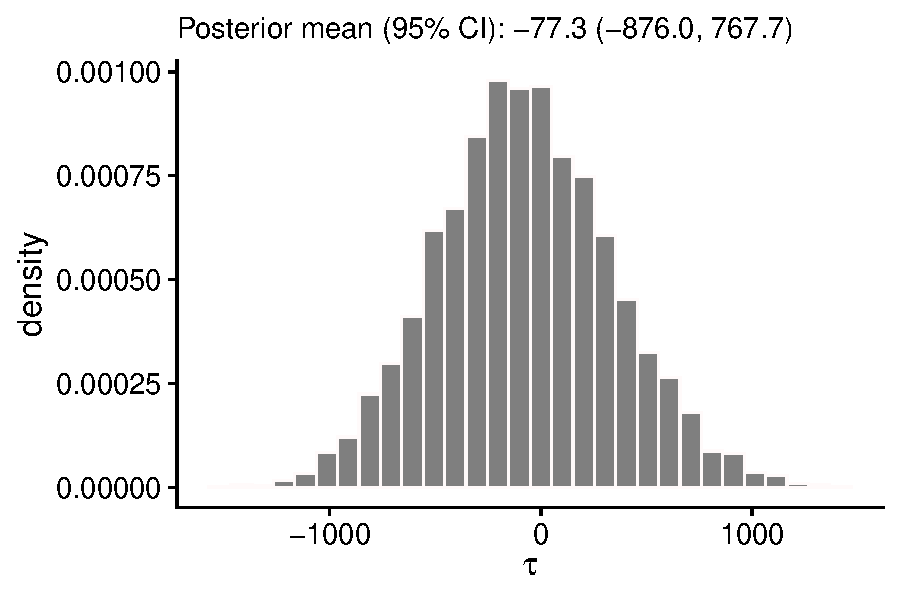
\includegraphics[width=0.7\textwidth]{figures/tauplot.pdf}
    \caption{\label{fig:tauplot} Posterior distribution for average
      treatment effect $\tau$ }
  \end{figure}


\end{enumerate}

%%% Local Variables:
%%% mode: latex
%%% TeX-master: "../main"
%%% End:
